\subsection{Kullback Leibler Divergence}

\subsubsection{The formula}
The \emph{Kullback-Leibler} (KL) Divergence is not, as its name indicates it, a mesure of a distance between subsets of the corpus, but it is a divergence between them. Indeed, let us consider sets $P$ and $Q$ containing articles for one year each. The KL divergence is defined as follows :

\begin{eqnarray}\label{KL}
    D_{KL}(P||Q) = \sum_i P(i) ln \frac{P(i)}{Q(i)}
\end{eqnarray}

It computes the sum of multiplications between the probability of the word $i$ in corpus $P$ and the natural logarithm of the same probability over the probability of the word $i$ in $Q$. Thus, $P$ and $Q$ need to be vectors containing the same words at the same indexes. We also can explain the \emph{Kullback-Leibler} Divergence as the lost when $Q$ is used to approximate $P$ or, in other words, as the fact that $Q$ tries to simulate $P$.

Obviously, this divergence is not symmetric. Indeed, let us take for example two years $y_1$ and $y_2$ from the corpus. Suppose now that $y_1$ contains more common words than $y_2$, that contains more uncommon words. We can conclude that $y_2$ will have a better approximation of $y_1$ than $y_1$ with $y_2$. This is only because $y_2$ has a bigger subset of words of $y_1$, so it can simulate it easily. We can observe this phenomenon in the following plots. The years around 1840 have some difficulties to simulate 1990's years but in the other direction it is easy because there is more vocabulary in the 20th century than in the 19th.\\

To compute this formula, as we need to have vectors with the same size representing the same words in the same order and as some words appear only in certain year, it is needed to add the missing words in each year with a number of occurrences equal to 0. Doing so, we have for each year a vector containing all words over the whole corpus. With KL Divergence, we have to be careful, because if $P(i)$ or $Q(i)$ is 0, the computation will be totally wrong. Thus, we have to add some smoothing in the KL computation. We made the choice to add a really small value ($10^{25}$) and to weight it with the probability of the word over the whole corpus. Thus, we keep a small difference between words that appear a lot in the corpus and the one that appear not so much\footnote{It is a way to have less consideration for word that appear not so much, like words that does not exist in french and that we were not be able to correct perfectly.}.

\subsubsection{Computation of \emph{Kullback-Leibler} Divergence}
We computed the \emph{Kullback-Leibler} Divergence with the non-corrected corpus and the OCR-corrected corpus and also using the probability that a word appear in a year and the TF-IDF value of each word. The explanations about the plots are located below.

\begin{figure}[h!]
    \begin{minipage}[b]{0.48\linewidth}
        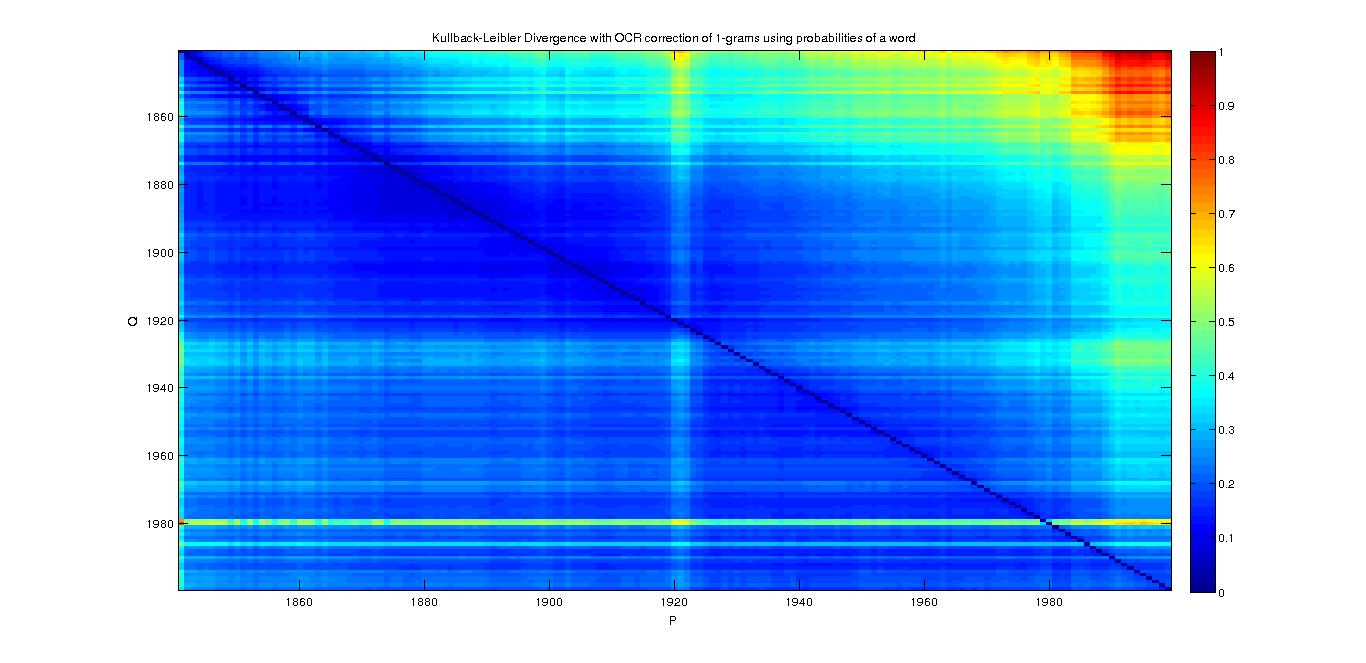
\includegraphics[scale=0.15]{Pictures/kullback-leibler/KL_1-grams_with_correction_proba.jpg}
        \caption{KL for 1-gram with OCR correction and probability of word}
        \label{KL-PC1}
    \end{minipage}\hfill
    \begin{minipage}[b]{0.5\linewidth}
        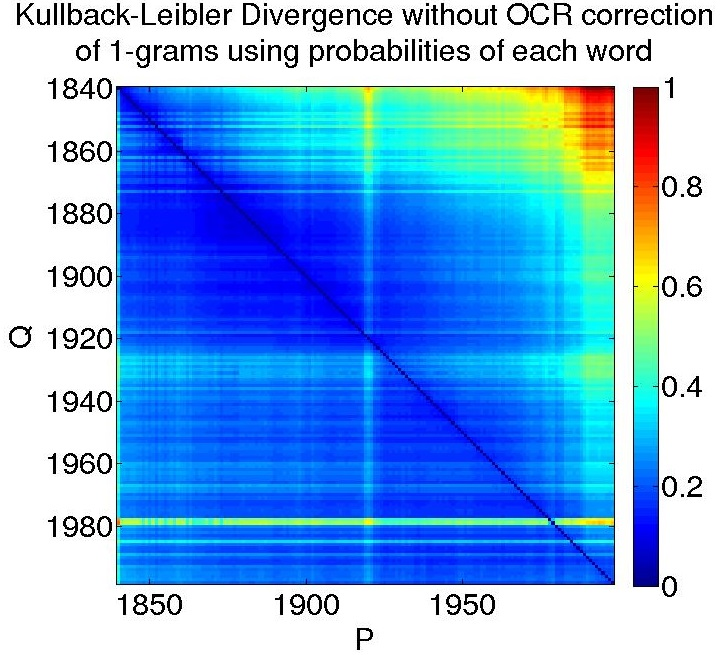
\includegraphics[scale=0.15]{Pictures/kullback-leibler/KL_1-grams_without_correction_proba.jpg}
        \caption{KL for 1-gram without OCR correction and probability of word}
        \label{KL-PN1}
    \end{minipage}\hfill
\end{figure}

\begin{figure}[h!]
    \begin{minipage}[b]{0.48\linewidth}
        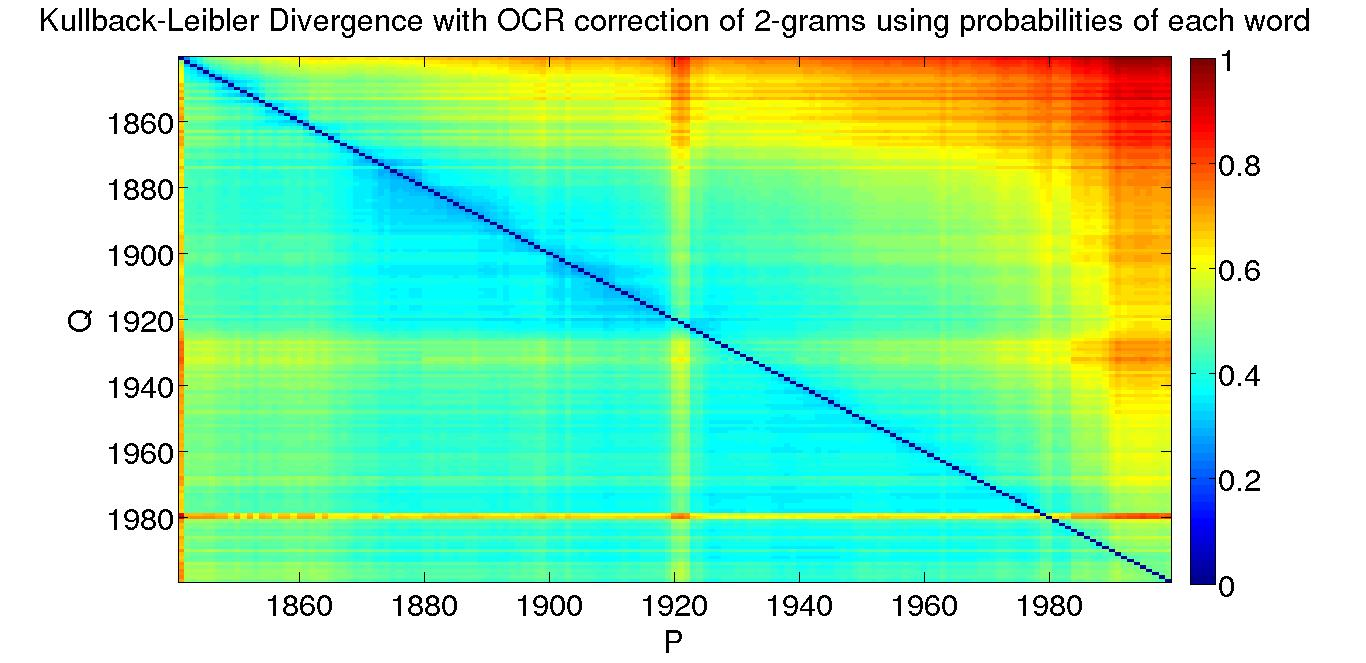
\includegraphics[scale=0.15]{Pictures/kullback-leibler/KL_2-grams_with_correction_proba.jpg}
        \caption{KL for 2-grams with OCR correction and probability of word}
        \label{KL-PC2}
    \end{minipage}\hfill
    \begin{minipage}[b]{0.5\linewidth}
        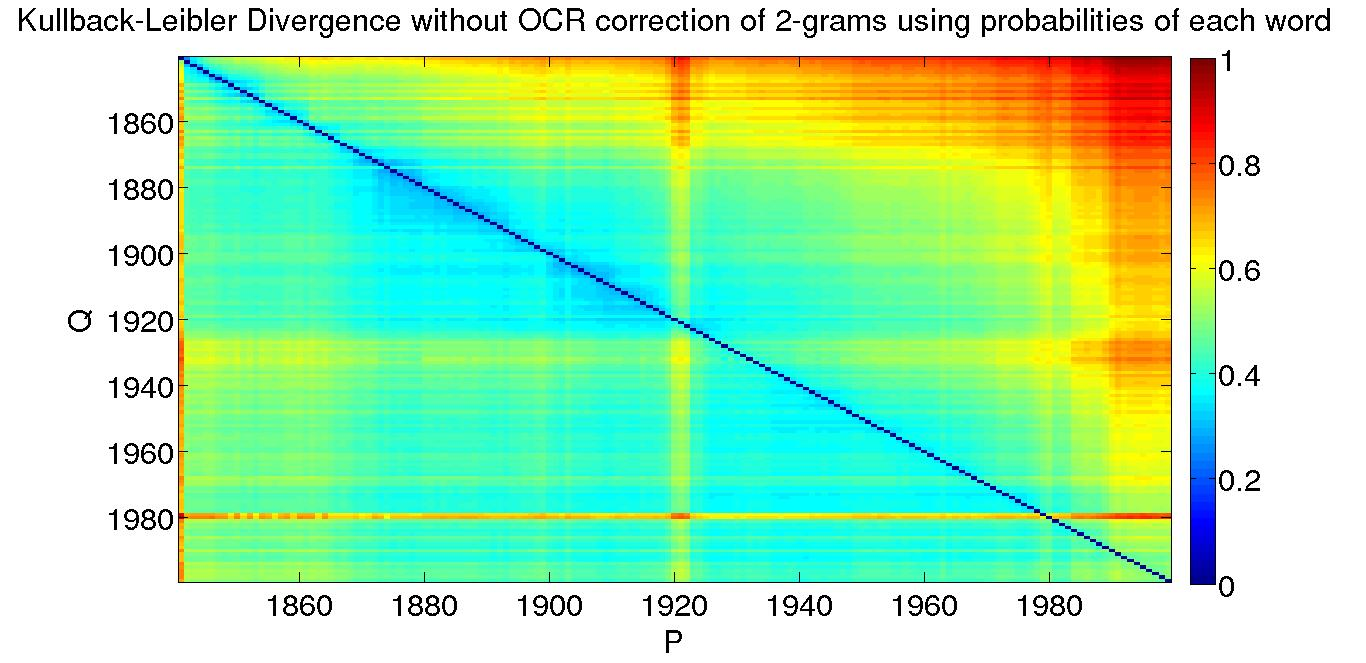
\includegraphics[scale=0.15]{Pictures/kullback-leibler/KL_2-grams_without_correction_proba.jpg}
        \caption{KL for 2-grams without OCR correction and probability of word}
        \label{KL-PN2}
    \end{minipage}\hfill
\end{figure}

\begin{figure}[h!]
    \begin{minipage}[b]{0.48\linewidth}
        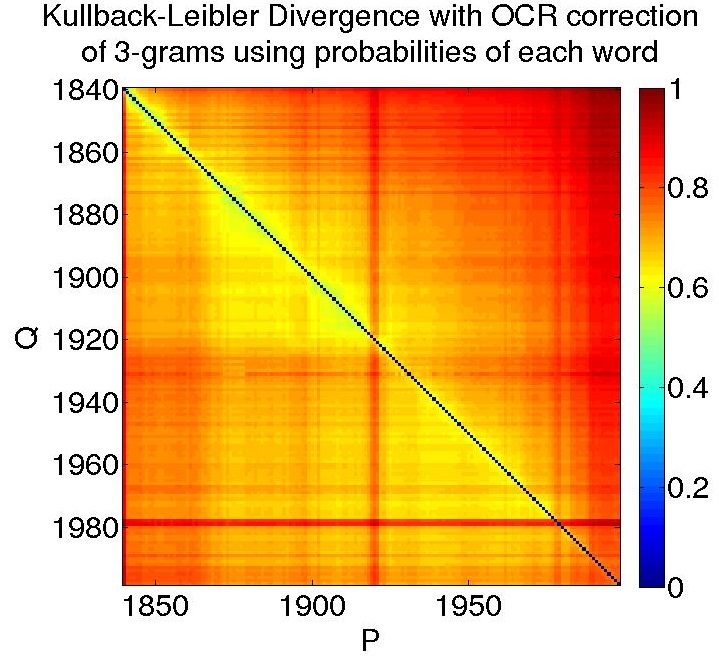
\includegraphics[scale=0.15]{Pictures/kullback-leibler/KL_3-grams_with_correction_proba.jpg}
        \caption{KL for 3-grams with OCR correction and probability of word}
        \label{KL-PC3}
    \end{minipage}\hfill
    \begin{minipage}[b]{0.5\linewidth}
        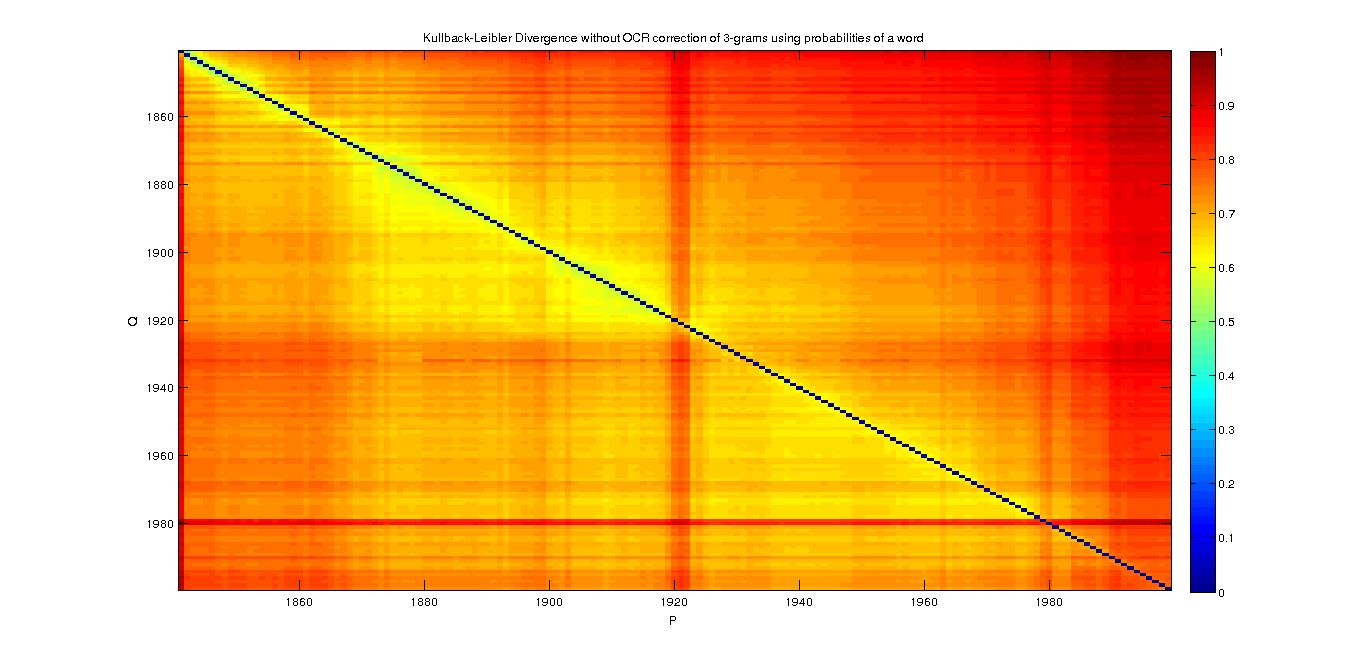
\includegraphics[scale=0.15]{Pictures/kullback-leibler/KL_3-grams_without_correction_proba.jpg}
        \caption{KL for 3-grams without OCR correction and probability of word}
        \label{KL-PN3}
    \end{minipage}\hfill
\end{figure}

\begin{figure}[h!]
    \begin{minipage}[b]{0.48\linewidth}
        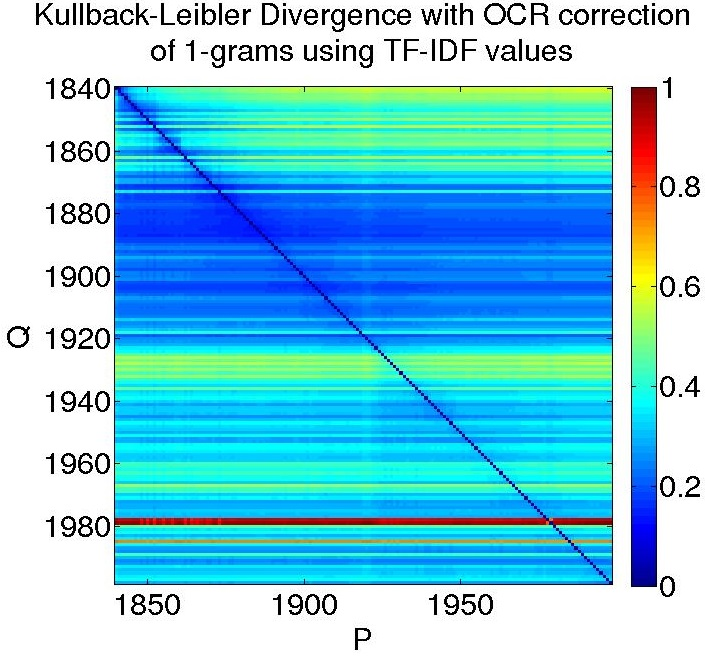
\includegraphics[scale=0.15]{Pictures/kullback-leibler/KL_1-grams_with_correction_tfidf.jpg}
        \caption{KL for 1-gram with OCR correction and TF-IDF}
        \label{KL-TC1}
    \end{minipage}\hfill
    \begin{minipage}[b]{0.5\linewidth}
        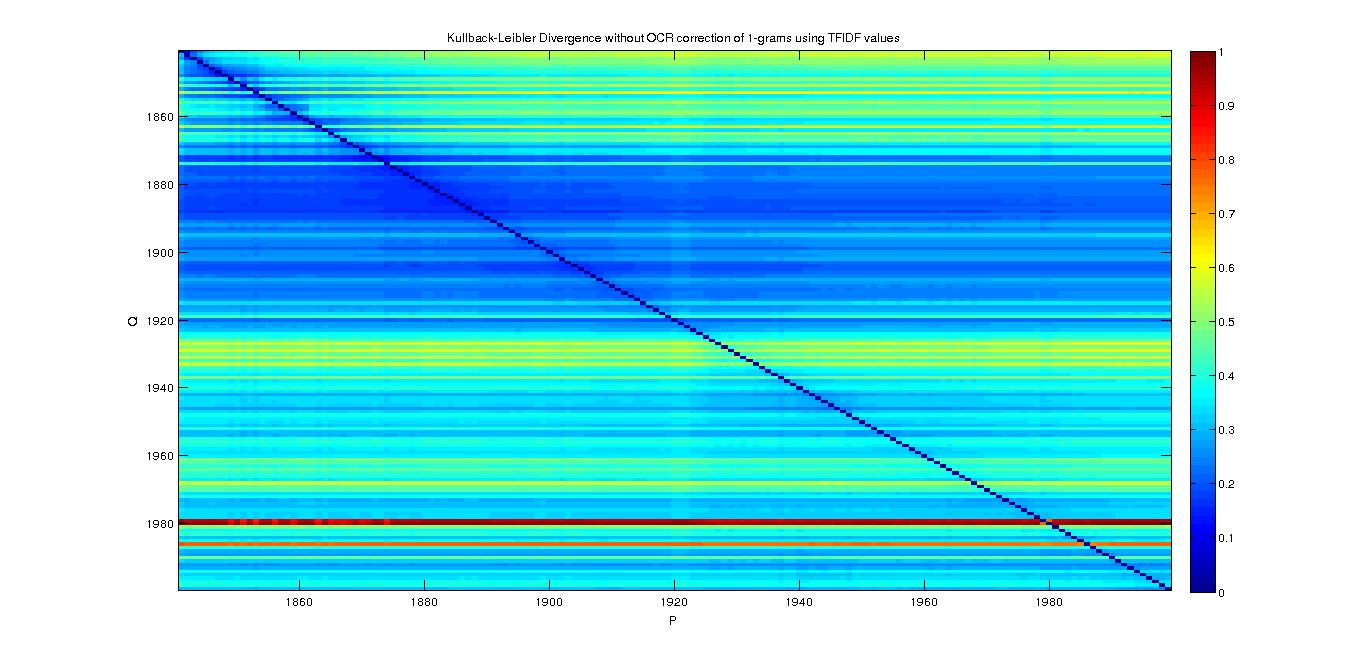
\includegraphics[scale=0.15]{Pictures/kullback-leibler/KL_1-grams_without_correction_tfidf.jpg}
        \caption{KL for 1-gram without OCR correction and TF-IDF}
        \label{KL-TN1}
    \end{minipage}\hfill
\end{figure}

\begin{figure}[h!]
    \begin{minipage}[b]{0.48\linewidth}
        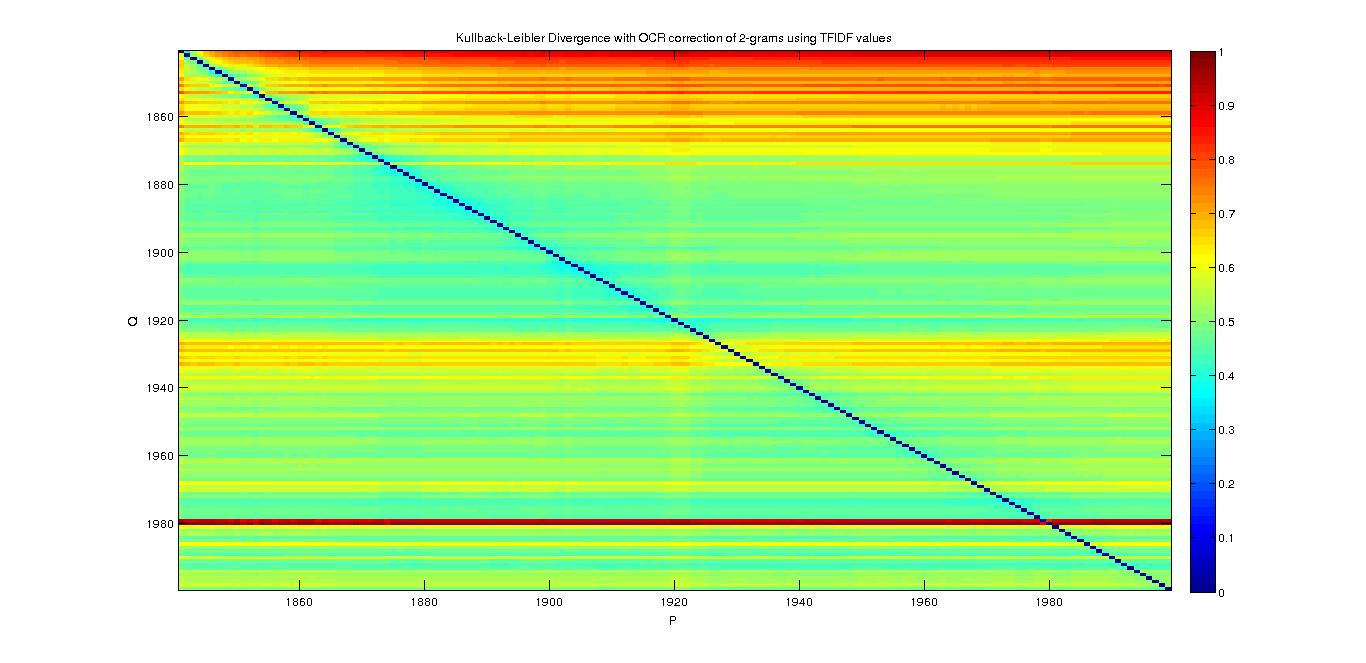
\includegraphics[scale=0.15]{Pictures/kullback-leibler/KL_2-grams_with_correction_tfidf.jpg}
        \caption{KL for 2-grams with OCR correction and TF-IDF}
        \label{KL-TC2}
    \end{minipage}\hfill
    \begin{minipage}[b]{0.5\linewidth}
        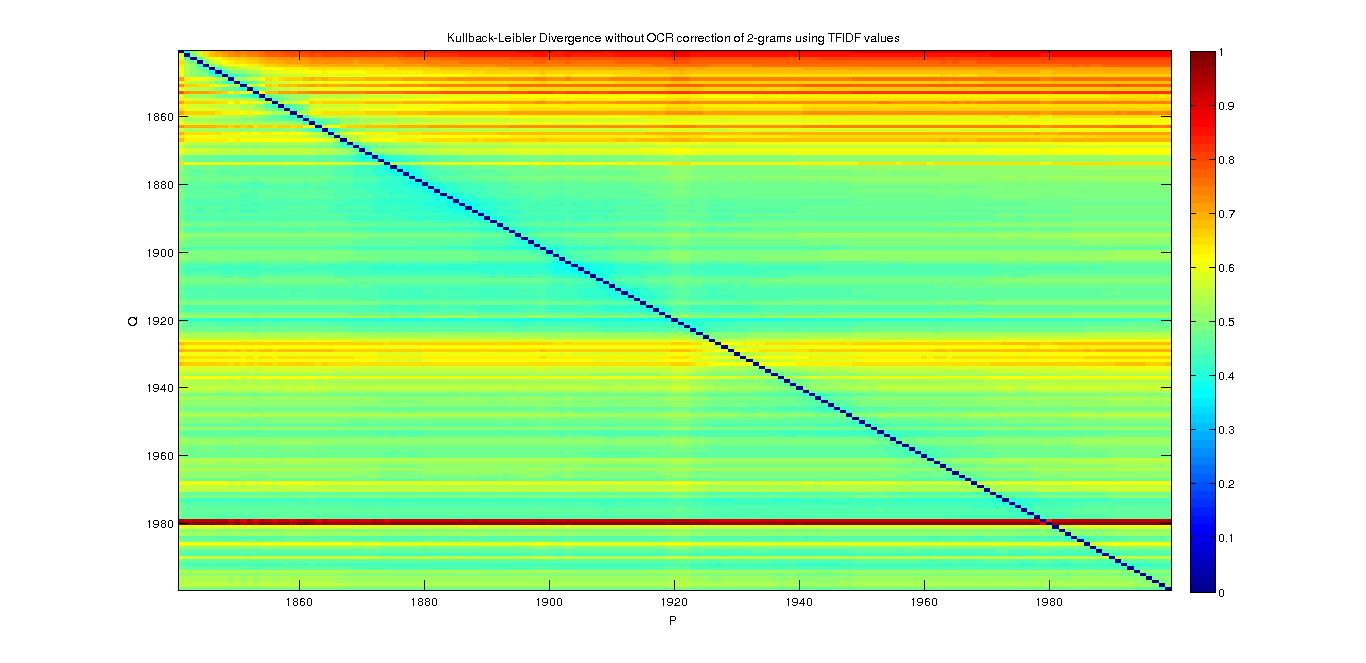
\includegraphics[scale=0.15]{Pictures/kullback-leibler/KL_2-grams_without_correction_tfidf.jpg}
        \caption{KL for 2-grams without OCR correction and TF-IDF}
        \label{KL-TN2}
    \end{minipage}\hfill
\end{figure}

\begin{figure}[h!]
    \begin{minipage}[b]{0.48\linewidth}
        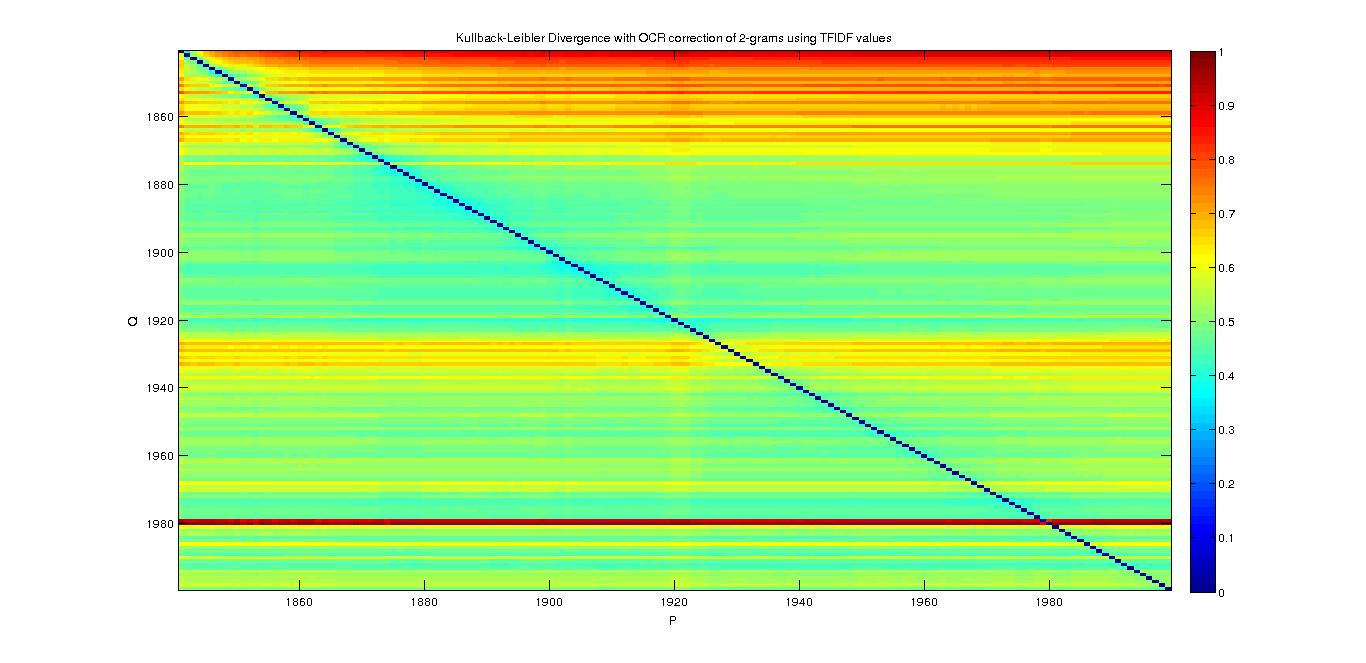
\includegraphics[scale=0.15]{Pictures/kullback-leibler/KL_2-grams_with_correction_tfidf.jpg}
        \caption{KL for 3-grams with OCR correction and TF-IDF}
        \label{KL-TC3}
    \end{minipage}\hfill
    \begin{minipage}[b]{0.5\linewidth}
        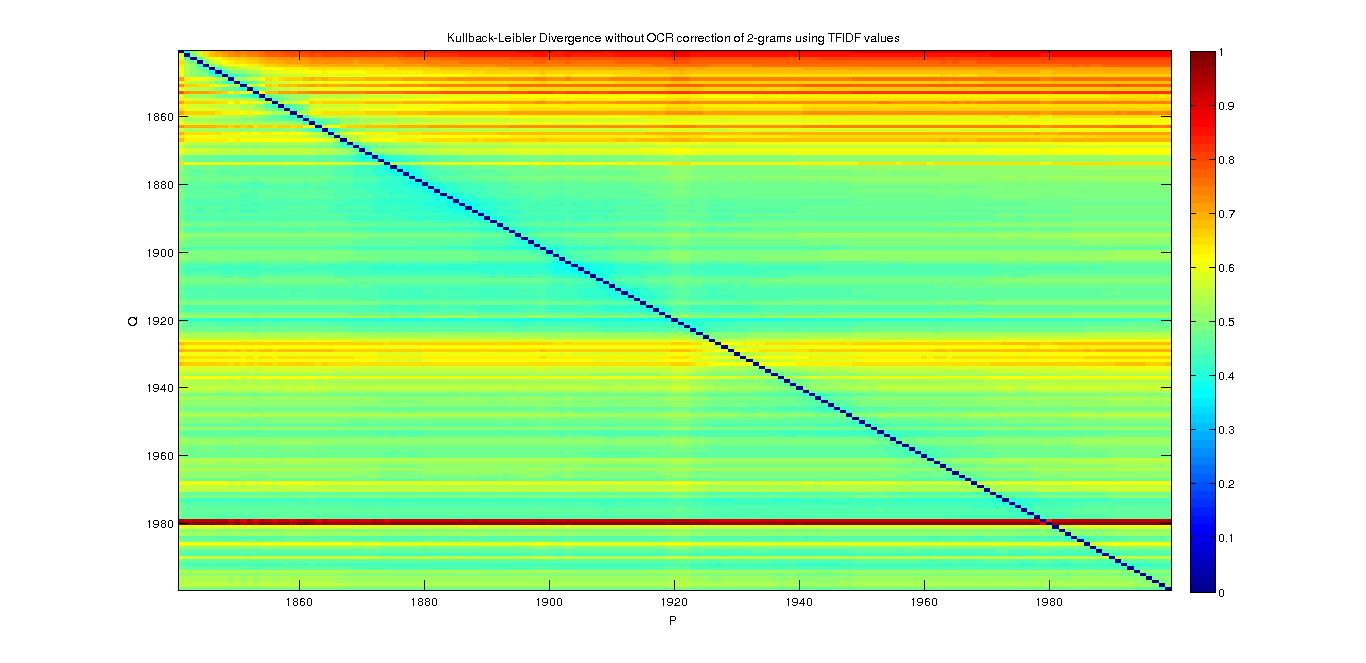
\includegraphics[scale=0.15]{Pictures/kullback-leibler/KL_2-grams_without_correction_tfidf.jpg}
        \caption{KL for 3-grams without OCR correction and TF-IDF}
        \label{KL-TN3}
    \end{minipage}\hfill
\end{figure}

\subsubsection{Analysis of results}
As we can observe, there is no real difference between the non-corrected corpus and the corrected one. Thus, we can assume that the OCR correction is not really helping to compute the distance between articles from each year. The interesting fact is that the upper right corner in each plot with the probability of a word (figures \ref{KL-PC1} to \ref{KL-PN3}) has a higher divergence value than the rest of the plot. It is, as explained in the section of this report about synonyms, because the trend is to increase the number of words and not to the disappearance of them. Indeed, if we have less words in 1840 and much more in 1998, it is obvious that when we approximate 1840 with 1998, the divergence is low and when we approximate 1998 with 1840 it is more difficult (right upper corner).

Augmenting the degree of n-grams, we can observe that, generally, the plots become more red because the divergence is bigger, which is totally understandable (we have n-grams that occur less, so it the approximation of a year with another one becomes more difficult). With the 2-grams, the "red part" is larger in the right upper corner and with the 3-grams, all the plot becomes red. In the 3-grams plot, we can also see that there is a light tight band around the diagonal, which indicates us that the articles from close years share a bigger set of words.

The results of \emph{Kullback-Leibler} divergence with TF-IDF (figures \ref{KL-TC1} to \ref{KL-TN3}) are really strange and have always the same form (for 1,2 and 3-grams). It is difficult to explain why it has this form, but a possible explanation is that the TF-IDF gives more importance to the words that appears less in the corpus. Knowing that we try to approximate a year with another one, it is obvious that it becomes difficult to approximate a year if the uncommon words have more weight. It can explain the lines in the plots, because a year could have the same difficulties to approximate each other years.